\documentclass[fleqn,compress,utf8,aspectratio=169,t]{beamer}
\usetheme{LMU}
% Prevent slide breaks in the middle of a paragraph
\widowpenalties 1 10000
\raggedbottom

\makeatletter
\@ifundefined{KOMAClassName}{% if non-KOMA class
  \IfFileExists{parskip.sty}{%
    \RequirePackage{parskip}
  }{% else
    \setlength{\parindent}{0pt}
    \setlength{\parskip}{6pt plus 2pt minus 1pt}}
}{% if KOMA class
  \KOMAoptions{parskip=half}}
\makeatother

\IfFileExists{xurl.sty}{\usepackage{xurl}}{} % add URL line breaks if available
\IfFileExists{bookmark.sty}{\usepackage{bookmark}}{\usepackage{hyperref}}
\urlstyle{same} % disable monospaced font for URLs

\usepackage{listings}
\lstset{defaultdialect=[5.3]Lua}
\lstset{defaultdialect=[x86masm]Assembler}
\usepackage{longtable,booktabs}
\usepackage{caption}
% Make caption package work with longtable
\makeatletter
\def\fnum@table{\tablename~\thetable}
\makeatother
\usepackage{graphicx}
\makeatletter
\def\maxwidth{\ifdim\Gin@nat@width>\linewidth\linewidth\else\Gin@nat@width\fi}
\def\maxheight{\ifdim\Gin@nat@height>\textheight\textheight\else\Gin@nat@height\fi}
\makeatother
% Scale images if necessary, so that they will not overflow the page
% margins by default, and it is still possible to overwrite the defaults
% using explicit options in \includegraphics[width, height, ...]{}
\setkeys{Gin}{width=\maxwidth,height=\maxheight,keepaspectratio}
% Set default figure placement to htbp
\makeatletter
\def\fps@figure{htbp}
\makeatother
\usepackage[normalem]{ulem}
% Avoid problems with \sout in headers with hyperref
\pdfstringdefDisableCommands{\renewcommand{\sout}{}}
\setlength{\emergencystretch}{3em} % prevent overfull lines
%Tightlist Command
\providecommand{\tightlist}{%
  \setlength{\itemsep}{0pt}\setlength{\parskip}{0pt}}



\usepackage[ngerman]{babel}
\usepackage[style=ieee]{biblatex}
\usepackage{pifont}
\usepackage{subcaption}
\usepackage{tikz}
\usetikzlibrary{backgrounds,calc,decorations.pathreplacing,positioning}
\addbibresource{Abschlussvortrag.bib}

%%%%%%%%%%%%%%%%%%%%%%%%%%%%%%%%%%%%%%%%%%%%%%%%%%%%%%%%%%%%%%%%%%%%%%%%%%%%%%%%
%%                                 Customizations                             %%
%%%%%%%%%%%%%%%%%%%%%%%%%%%%%%%%%%%%%%%%%%%%%%%%%%%%%%%%%%%%%%%%%%%%%%%%%%%%%%%%

% If you want no navigation uncomment this
%\beamertemplatenavigationsymbolsempty

% setup listings
\lstset{
  basicstyle=\ttfamily\color{black},
  showstringspaces=false
}

\lstdefinestyle{highlight}{
  keywordstyle=\color{red},
  commentstyle=\color{lmu@darkgray}
}

\lstdefinestyle{basetex}{
language={[LaTeX]Tex},
basicstyle=\color{black!40},
keywordstyle=\color{red!40},
commentstyle=\color{lmu@darkgray!40},
moredelim=**[il][\only<+>{\color{black}\lstset{style=highlight}}]{@}
}

\lstdefinestyle{basec}{
language=C,
basicstyle=\color{black!40},
keywordstyle=\color{red!40},
commentstyle=\color{green!40},
moredelim=**[il][\only<+>{\color{black}\lstset{style=highlight}}]{@}
}

%%%%%%%%%%%%%%%%%%%%%%%%%%%%%%%%%%%%%%%%%%%%%%%%%%%%%%%%%%%%%%%%%%%%%%%%%%%%%%%%
%%                                  Title Page Data                           %%
%%%%%%%%%%%%%%%%%%%%%%%%%%%%%%%%%%%%%%%%%%%%%%%%%%%%%%%%%%%%%%%%%%%%%%%%%%%%%%%%
% helper command to add multiple authors
\newcommand{\newauthor}[2]{
\parbox[c]{0.26\textwidth}{
{\bfseries #1} \\
{\scriptsize{\href{mailto:#2}{#2}}}
}
}

\author[Uffmann]{
  \newauthor{Adrian Uffmann}{adrian.uffmann@campus.lmu.de}
}

\institute[LMU]{
  {LMU München}
}

\date[1.2.22]{01.02.2022}

\title{Entwicklung leistungsfähiger RMA-Locks durch Portierung und Optimierung von NUMA-Algorithmen}
\subtitle{Abschlussvortrag Masterarbeit}

\hypersetup{
  pdftitle={Title},
  pdfauthor={Author},
  hidelinks}

%%%%%%%%%%%%%%%%%%%%%%%%%%%%%%%%%%%%%%%%%%%%%%%%%%%%%%%%%%%%%%%%%%%%%%%%%%%%%%%%
%%                                  Document                                  %%
%%%%%%%%%%%%%%%%%%%%%%%%%%%%%%%%%%%%%%%%%%%%%%%%%%%%%%%%%%%%%%%%%%%%%%%%%%%%%%%%

\begin{document}

\begin{frame}
    \titlepage
\end{frame}

\section{Einführung}

\begin{frame}{Motivation}
    \begin{itemize}
        \item Locks sind einer der wichtigsten Grundbausteine zur Synchronisierung in parallelen Programmen
        \item Es gibt viele Lock-Algorithmen für gemeinsamen Speicher
              %   \begin{itemize}
              %       \item RH-Lock \cite{RH-Lock},
              %             HCLH-Lock \cite{HCLH-Lock},
              %             % FC-MCS-Lock \cite{FC-MCS-Lock},
              %             Cohort-Lock \cite{Cohort-Lock},
              %             HMCS-Lock \cite{HMCS-Lock},
              %             AHMCS-Lock \cite{AHMCS-Lock},
              %             CST-Lock \cite{CST-Lock},
              %             % CNA-Lock \cite{CNA-Lock},
              %             SHFL-Lock \cite{SHFL-Lock},
              %             ...
              %   \end{itemize}
        \item Aber kaum welche für verteilten Speicher
              \begin{itemize}
                  \item \texttt{MPI\_Win\_lock}
                  \item \texttt{dash::Mutex} \cite{DART-MPI}
                  \item D-MCS und RMA-MCS \cite{RMA-RW}
              \end{itemize}
    \end{itemize}
\end{frame}

\begin{frame}{Gemeinsamer und verteilter Speicher}
    \begin{itemize}
        \item MPI bietet mit \textit{Remote Memory Access} (RMA) einseitige Kommunikation für verteilten Speicher an, die sehr ähnlich zu gemeinsamem Speicher ist:
              \begin{itemize}
                  \item Lesender Zugriff (MPI\_Get)
                  \item Schreibender Zugriff (MPI\_Put)
                  \item Atomarer Zugriff (MPI\_Accumulate, MPI\_Get\_accumulate, MPI\_Compare\_and\_swap, ...)
              \end{itemize}\pause
        \item Zugriffe auf entfernten Speicher haben eine hohe Latenz
        \item[$\Rightarrow$] Zugriffe auf entfernten Speicher müssen vermieden werden
    \end{itemize}
\end{frame}

\begin{frame}
    \begin{itemize}
        \item[$\Rightarrow$] Zugriffe auf entfernten Speicher müssen vermieden werden
    \end{itemize}
    Das gibt es auch auf gemeinsamem Speicher ... \pause bei NUMA
    \vfill

    \tikzstyle{mem} = [rectangle, draw, color=blue, fill=blue!20, text centered, rounded corners]
    \tikzstyle{cpu} = [rectangle, draw, color=red, fill=red!20, text centered]
    \tikzstyle{mem-access} = [draw, color=black, -latex]
    \tikzstyle{cpu-connect} = [draw, color=black]
    \tikzstyle{numa-node} = [draw, color=gray, fill=gray!20]
    \begin{minipage}[b]{.49\textwidth}
        \begin{figure}
            \centering
            \begin{tikzpicture}[node distance = 4.5em]
                \node [cpu] (uma-cpu-1) {CPU};
                \node [cpu, right of=uma-cpu-1] (uma-cpu-2) {CPU};
                \node [cpu, right of=uma-cpu-2] (uma-cpu-3) {CPU};
                \node [cpu, right of=uma-cpu-3] (uma-cpu-4) {CPU};
                \node [mem, below = of $(uma-cpu-2)!0.5!(uma-cpu-3)$] (uma-mem) {Mem};

                \path [mem-access] (uma-cpu-1) |- ++(0, -2.5em) -| (uma-mem);
                \path [mem-access] (uma-cpu-2) |- ++(0, -2.5em) -| (uma-mem);
                \path [mem-access] (uma-cpu-3) |- ++(0, -2.5em) -| (uma-mem);
                \path [mem-access] (uma-cpu-4) |- ++(0, -2.5em) -| (uma-mem);
            \end{tikzpicture}
            \caption{Uniform Memory Access}
        \end{figure}
    \end{minipage}
    \begin{minipage}[b]{.49\textwidth}
        \begin{figure}
            \centering
            \begin{tikzpicture}[node distance = 4.5em]
                \node [mem] (numa-mem-1) {Mem};
                \node [cpu, right of=numa-mem-1] (numa-cpu-1) {CPU};
                \node [cpu, right of=numa-cpu-1] (numa-cpu-2) {CPU};
                \node [mem, right of=numa-cpu-2] (numa-mem-2) {Mem};
                \node [mem, below of=numa-mem-1] (numa-mem-4) {Mem};
                \node [cpu, below of=numa-cpu-1] (numa-cpu-4) {CPU};
                \node [cpu, below of=numa-cpu-2] (numa-cpu-3) {CPU};
                \node [mem, below of=numa-mem-2] (numa-mem-3) {Mem};

                \scoped[on background layer]{\filldraw [numa-node] ($(numa-mem-1)+(-0.75,0.75)$) rectangle ($(numa-cpu-1)+(0.75,-0.75)$);}
                \scoped[on background layer]{\filldraw [numa-node] ($(numa-cpu-2)+(-0.75,0.75)$) rectangle ($(numa-mem-2)+(0.75,-0.75)$);}
                \scoped[on background layer]{\filldraw [numa-node] ($(numa-cpu-3)+(-0.75,0.75)$) rectangle ($(numa-mem-3)+(0.75,-0.75)$);}
                \scoped[on background layer]{\filldraw [numa-node] ($(numa-mem-4)+(-0.75,0.75)$) rectangle ($(numa-cpu-4)+(0.75,-0.75)$);}

                \path [mem-access] (numa-cpu-1) -- (numa-mem-1);
                \path [mem-access] (numa-cpu-2) -- (numa-mem-2);
                \path [mem-access] (numa-cpu-3) -- (numa-mem-3);
                \path [mem-access] (numa-cpu-4) -- (numa-mem-4);
                \path [cpu-connect] (numa-cpu-1) -- (numa-cpu-2);
                \path [cpu-connect] (numa-cpu-2) -- (numa-cpu-3);
                \path [cpu-connect] (numa-cpu-3) -- (numa-cpu-4);
                \path [cpu-connect] (numa-cpu-4) -- (numa-cpu-1);
            \end{tikzpicture}
            \caption{Non-Uniform Memory Access}
        \end{figure}
    \end{minipage}
\end{frame}

\begin{frame}{Forschungsfrage}
    \vfill
    Können Lock-Algorithmen für NUMA-Systeme auf verteilten Speicher portiert werden,
    um eine bessere Performance als bestehende Implementierungen verteilter Locks zu erreichen?
    \vfill
\end{frame}

\begin{frame}{Themenverwandte Arbeit}
    Es gibt hierzu bereits eine Arbeit von \citeauthor{RMA-RW}~\cite{RMA-RW}:
    \begin{itemize}
        \item Stellt hierarchischen Lock für verteilten Speicher vor: RMA-MCS
        \item Basiert auf einem Lock-Algorithmus für NUMA: HMCS-Lock \cite{HMCS-Lock}
        \item Nutzt foMPI~\cite{foMPI}\pause
              \begin{itemize}
                  \item foMPI funktioniert nur auf Cray Gemini (XK5, XE6) und Aries (XC30) Systemen\pause
                  \item RMA-MCS bewegt sich außerhalb der Garantien von MPI 3.1 \cite[Kapitel 11.7.3]{MPI-3.1}
                  \item[$\Rightarrow$] Portierung auf Intel-MPI war schwierig
              \end{itemize}
    \end{itemize}
\end{frame}

\section{Übersicht}

\begin{frame}{Übersicht über den weiteren Vortrag}
    \begin{itemize}
        \item Benchmarks
        \item Optimierung der Basislocks
        \item Portierung von NUMA-Locks
        \item Fazit
    \end{itemize}
\end{frame}

\section{Benchmarks}

\begin{frame}{Benchmarks}
    \begin{itemize}
        \item Benchmarks aus themenverwandter Arbeit \cite{RMA-RW} fokussieren \textit{Reader}-\textit{Writer}-Locks
        \item Sonst keine Benchmarks verfügbar\pause
        \item[$\Rightarrow$] Neue Benchmarksuite erforderlich
    \end{itemize}
\end{frame}

\begin{frame}{Kennzahlen}
    \begin{itemize}
        \item Geschwindigkeit
        \item Konkurrenz
              \begin{itemize}
                  \item<2-> Definition: Der Anteil
                        der Akquisitionen, bei denen ein Prozess den Lock nicht direkt akquirieren konnte, sondern
                        auf einen Vorgänger warten musste.
              \end{itemize}
        \item Fairness\pause
              \begin{itemize}
                  \item<3-> Nicht die theoretische Fairness des Algorithmus
                  \item<3-> Sondern die praktische Fairness der Implementierung (wie in \cite{Cohort-Lock})
                  \item<3->[$\Rightarrow$] Variationskoeffizient (CV) des Prozessfortschritts
              \end{itemize}
              % \item Weitere algorithmusspezifische Kennzahlen
    \end{itemize}
\end{frame}

\begin{frame}{Benchmarksuite}
    \begin{itemize}
        \item \textit{Uncontested Performance Benchmark} (UPB)
              \begin{itemize}
                  \item[$\Rightarrow$] 0~\% Konkurrenz
              \end{itemize}
        \item \textit{Empty Critical Section Benchmark} (ECSB)
              \begin{itemize}
                  \item[$\Rightarrow$] 100~\% Konkurrenz
              \end{itemize}
        \item \textit{Wait Before Acquire Benchmark} (WBAB)
              \begin{itemize}
                  \item[$\Rightarrow$] Variable Konkurrenz von 100~\% bis 0~\%
              \end{itemize}
        \item \textit{Changing Critical Work Benchmark} (CCWB)
              \begin{itemize}
                  \item[$\Rightarrow$] Möglichst realistisch mit variabler Konkurrenz von 0~\% bis 100~\%
              \end{itemize}
    \end{itemize}
\end{frame}

\section{Optimierung der Basislocks}

\begin{frame}{\texttt{dash::Mutex}}
    \begin{itemize}
        \item Bestandteil der PGAS-Bibliothek DASH \cite{DART-MPI}
        \item Basiert auf dem MCS-Lock \cite{MCS-Lock}
        \item Nutzt Punkt-zu-Punkt-Kommunikation für Lockübergaben\\(\texttt{MPI\_Send} und \texttt{MPI\_Recv})
    \end{itemize}
\end{frame}

\begin{frame}{Optimierung von \texttt{dash::Mutex}}
    \begin{minipage}{.52\textwidth}
        \begin{itemize}
            \setlength\itemsep{.75em}
            \item Iterationsdauer $\Rightarrow$ Geringer ist besser
            \item Viel kritische Arbeit = Hohe Konkurrenz
            \item \texttt{dash::Mutex} ließ sich stark optimieren
        \end{itemize}
    \end{minipage}
    \begin{minipage}{.47\textwidth}
        \begin{figure}
            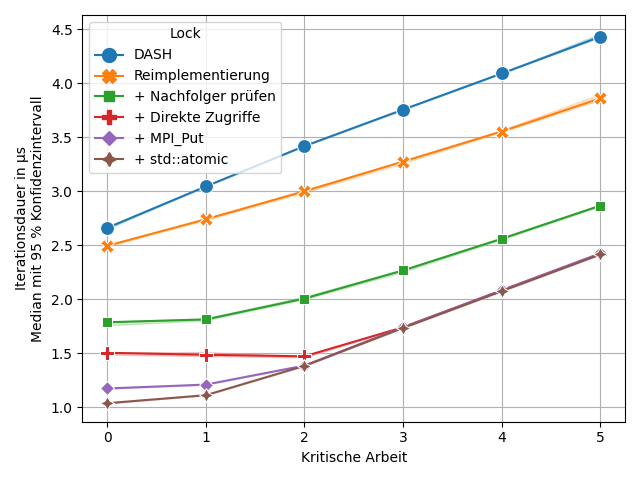
\includegraphics[width=\textwidth]{../../Dokumentation/Latex/Bilder/benchmarks/intelmpi/dash-optimization/CCWB-processes=28-latency}
            \caption{CCWB mit 28 Prozessen}
        \end{figure}
    \end{minipage}
\end{frame}

\begin{frame}{Optimierte Basislocks}
    \begin{minipage}{.49\textwidth}
        \begin{figure}
            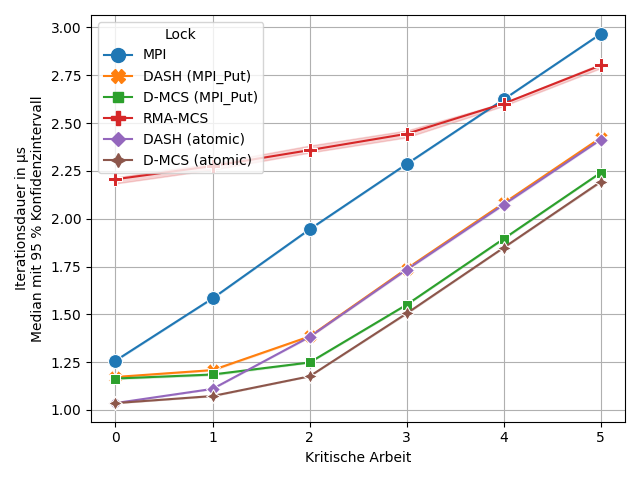
\includegraphics[width=\textwidth]{../../Dokumentation/Latex/Bilder/benchmarks/intelmpi/baseline-opt/CCWB-processes=28-latency}
            \caption{CCWB mit 28 Prozessen}
        \end{figure}
    \end{minipage}
    \begin{minipage}{.49\textwidth}
        \begin{figure}
            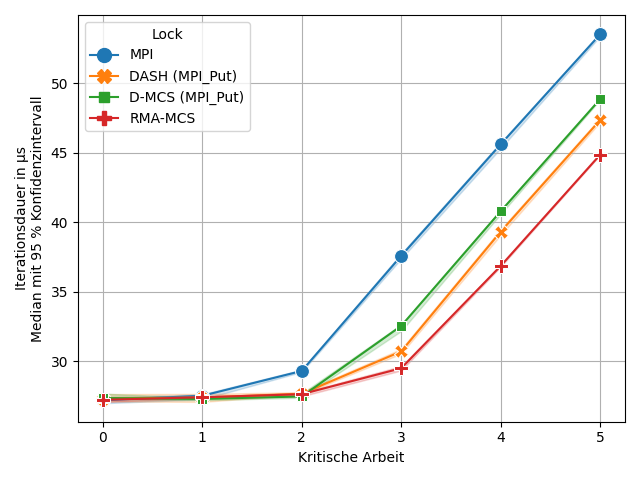
\includegraphics[width=\textwidth]{../../Dokumentation/Latex/Bilder/benchmarks/intelmpi/baseline-opt/CCWB-processes=112-latency}
            \caption{CCWB mit 112 Prozessen}
        \end{figure}
    \end{minipage}
\end{frame}

\section{Portierung von NUMA-Locks}

\begin{frame}{Betrachtete NUMA-Locks}
    \centering
    \begin{tabular}{|c|c|c|}
        \hline
        Algorithmus                    & Jahr & Geeignet  \\
        \hline
        RH-Lock \cite{RH-Lock}         & 2002 & \ding{52} \\
        \hline
        HCLH-Lock \cite{HCLH-Lock}     & 2006 & \ding{56} \\
        \hline
        Cohort-Lock \cite{Cohort-Lock} & 2012 & \ding{52} \\
        \hline
        HMCS-Lock \cite{HMCS-Lock}     & 2015 & \ding{56} \\
        \hline
        AHMCS-Lock \cite{AHMCS-Lock}   & 2016 & \ding{56} \\
        \hline
        CST-Lock \cite{CST-Lock}       & 2017 & \ding{56} \\
        \hline
        SHFL-Lock \cite{SHFL-Lock}     & 2019 & \ding{52} \\
        \hline
    \end{tabular}
\end{frame}

\begin{frame}{Cohort-Lock}
    \begin{itemize}
        \item Ein globaler Lock
        \item Ein lokaler Lock pro NUMA-Knoten
        \item Lokale Nachfolger ...
              \begin{itemize}
                  \item ... werden bevorzugt
                  \item ... erben globalen Lock automatisch
              \end{itemize}
        \item Verhinderung von \textit{Starvation} durch Zähler für lokale Lockübergaben
    \end{itemize}
\end{frame}

\begin{frame}{Cohort-Lock: Zähler-Optimierungen}
    \begin{minipage}{.52\textwidth}
        \begin{itemize}
            \setlength\itemsep{.5em}
            \item C-MCS-MCS = Cohort-Lock mit globalem und lokalen MCS-Lock
            \item Durchsatz $\Rightarrow$ Höher ist besser
            \item Wenig Wartezeit = Hohe Konkurrenz
            \item Direkte Portierung: langsam
            \item Mit Optimierung:
                  \vspace{.5em}
                  \begin{itemize}
                      \setlength\itemsep{.5em}
                      \item bis zu 8x so schnell wie zuvor
                      \item bis zu 4x so schnell wie RMA-MCS
                  \end{itemize}
        \end{itemize}
    \end{minipage}
    \begin{minipage}{.47\textwidth}
        \begin{figure}
            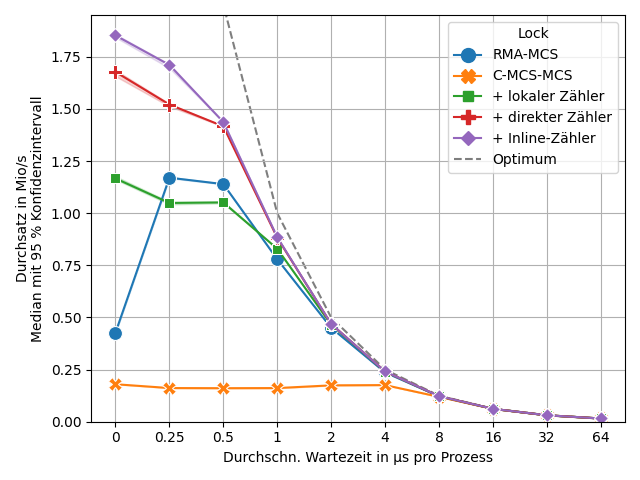
\includegraphics[width=\textwidth]{../../Dokumentation/Latex/Bilder/benchmarks/intelmpi/cohort-counter-optimization/WBAB-processes=112,mpi_progress=1-throughput}
            \caption{WBAB mit 112 Prozessen}
        \end{figure}
    \end{minipage}
\end{frame}

\begin{frame}{Cohort-Lock: Verschiedene globale und lokale Locks}
    \begin{itemize}
        \item Global:
              \begin{itemize}
                  \item TAS-Lock
                  \item MCS-Lock (optimierter \texttt{dash::Mutex})
                  \item TKT-Lock \cite{TKT-Lock}
              \end{itemize}
        \item Lokal:
              \begin{itemize}
                  \item MCS-Lock (optimierter D-MCS)
                  \item TKT-Lock \cite{TKT-Lock}
                  \item TTS-Lock
              \end{itemize}
    \end{itemize}
\end{frame}

\begin{frame}{Cohort-Lock: Evaluation verschiedener globaler und lokaler Locks}
    \begin{minipage}{.52\textwidth}
        \begin{itemize}
            \setlength\itemsep{.75em}
            \item Overhead = Iterationsdauer - Optimum
                  \vspace{.75em}
                  \begin{itemize}
                      \setlength\itemsep{.75em}
                      \item[$\Rightarrow$] Geringer ist besser
                  \end{itemize}
            \item<2-> Hohe Konkurrenz (0~\textmu{s} bis 0,5~\textmu{s}):
                  \vspace{.75em}
                  \begin{itemize}
                      \setlength\itemsep{.75em}
                      \item Lokaler Lock entscheidend
                      \item MCS am besten
                  \end{itemize}
            \item<3-> Mittlere Konkurrenz (1~\textmu{s} bis 4~\textmu{s}):
                  \vspace{.75em}
                  \begin{itemize}
                      \setlength\itemsep{.75em}
                      \item Globaler Lock entscheidend
                  \end{itemize}
        \end{itemize}
    \end{minipage}
    \begin{minipage}{.47\textwidth}
        \begin{figure}
            \begin{overprint}
                \onslide<1>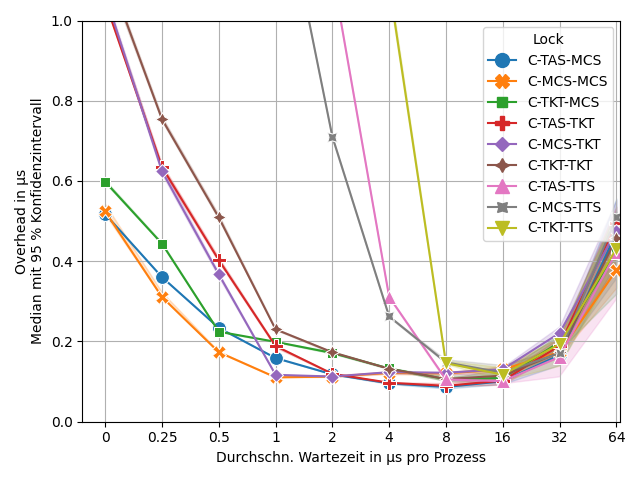
\includegraphics[width=\textwidth]{../../Dokumentation/Latex/Bilder/benchmarks/intelmpi/cohort-mcs-spin-tkt/WBAB-processes=112,mpi_progress=1-overhead}
                \onslide<2>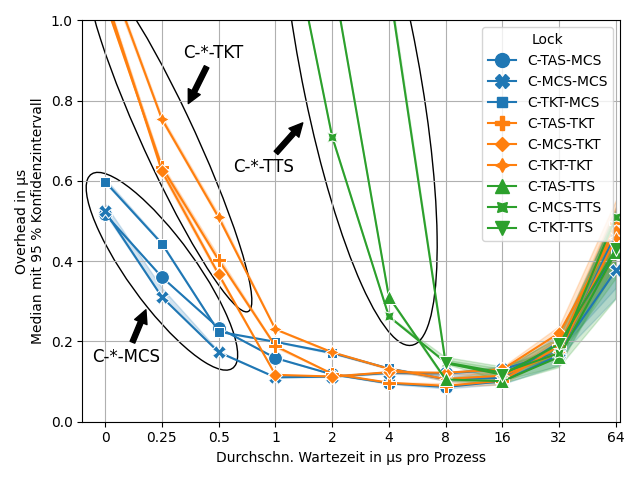
\includegraphics[width=\textwidth]{cohort-WBAB-112-overhead-low-contention}
                \onslide<3>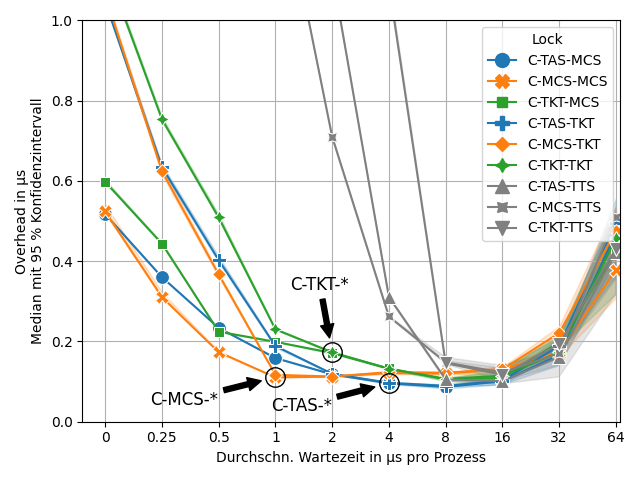
\includegraphics[width=\textwidth]{cohort-WBAB-112-overhead-medium-contention}
            \end{overprint}
            \caption{WBAB mit 112 Prozessen}
        \end{figure}
    \end{minipage}
\end{frame}

\begin{frame}{Cohort-Lock: Lokale Warteschlangen-Locks}
    \begin{itemize}
        \item Global:
              \begin{itemize}
                  \item MCS-Lock (optimierter \texttt{dash::Mutex})
              \end{itemize}
        \item Lokal:
              \begin{itemize}
                  \item MCS-Lock (optimierter D-MCS)
                  \item CLH-Lock \cite{C-Lock} \cite{LH-Lock}
                  \item Hemlock \cite{Hemlock}
              \end{itemize}
    \end{itemize}
\end{frame}

\begin{frame}{Cohort-Lock: Evaluation lokaler Warteschlangen-Locks}
    \begin{minipage}{.52\textwidth}
        \begin{itemize}
            \setlength\itemsep{.75em}
            \item Optimierungen aus Hemlock Arbeit \cite{Hemlock}:
                  \vspace{.75em}
                  \begin{itemize}
                      \setlength\itemsep{.75em}
                      \item Overlap
                      \item \textit{Coherence Traffic Reduction} (CTR)
                      \item \textit{Aggressive Hand-over} (AH)
                  \end{itemize}
            \item Optimierung aus HMCS Arbeit \cite{HMCS-Lock}:
                  \vspace{.75em}
                  \begin{itemize}
                      \setlength\itemsep{.75em}
                            \setlength\itemsep{.75em}
                      \item Inline-Zähler
                  \end{itemize}
            \item[$\Rightarrow$] Lokaler Hemlock am schnellsten
        \end{itemize}
    \end{minipage}
    \begin{minipage}{.47\textwidth}
        \begin{figure}
            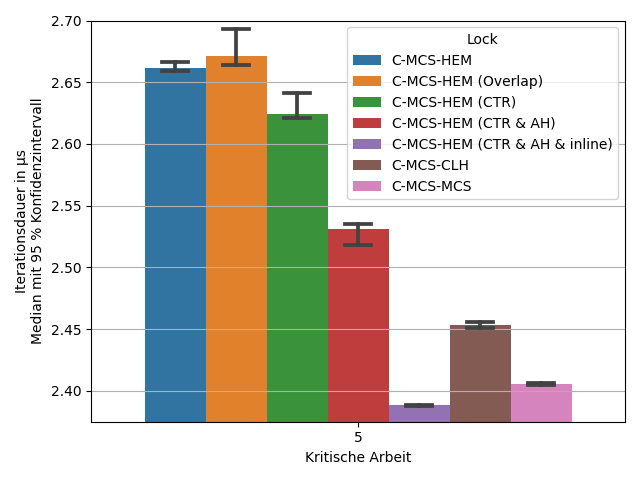
\includegraphics[width=\textwidth]{../../Dokumentation/Latex/Bilder/benchmarks/intelmpi/cohort-hem/CCWB-processes=28-latency-max}
            \caption{CCWB mit 28 Prozessen}
        \end{figure}
    \end{minipage}
\end{frame}

\section{Fazit}

\begin{frame}{Ergebnisse}
    \begin{itemize}
        \item C-MCS-HEM bis zu vier Mal so schnell wie RMA-MCS
              \begin{itemize}
                  \item Bei geringerem Speicherverbrauch
              \end{itemize}
        \item \texttt{dash::Mutex} konnte stark optimiert werden
              \begin{itemize}
                  \item Sollte trotzdem besser einen Algorithmus für NUMA nutzen
              \end{itemize}
        \item Neue Benchmarksuite
              \begin{itemize}
                  \item[$\Rightarrow$] Weitere Locks können leicht evaluiert werden
              \end{itemize}
    \end{itemize}
\end{frame}

\begin{frame}{Zukünftige Forschung}
    \begin{itemize}
        \item Untersuchung weiterer Algorithmen
              \begin{itemize}
                  \item FC-MCS \cite{FC-MCS-Lock}
                  \item CNA \cite{CNA-Lock}
                  \item Fissile-Locks \cite{Fissile-Locks}
                  \item CLoF \cite{CLoF}
              \end{itemize}
        \item Untersuchung von \textit{Reader}-\textit{Writer}-Locks
              \begin{itemize}
                  \item Kann für Implementierung von \texttt{MPI\_Win\_lock} genutzt werden
                  \item[$\Rightarrow$] Viele Anwendungen könnten profitieren
              \end{itemize}
    \end{itemize}
\end{frame}

\appendix

\section{References}

\begin{frame}[allowframebreaks]
    \frametitle{References}
    \nocite{*}
    \printbibliography[heading=none]
\end{frame}

\section{Optimierung}

\begin{frame}{Optimierung von \texttt{dash::Mutex}}
    \begin{minipage}{.49\textwidth}
        \begin{figure}
            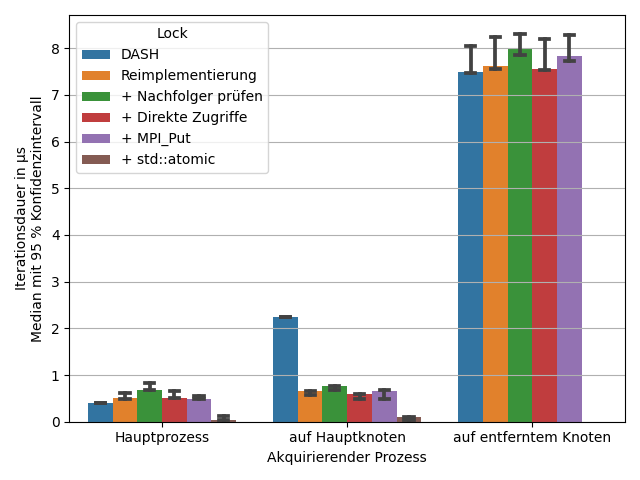
\includegraphics[width=\textwidth]{../../Dokumentation/Latex/Bilder/benchmarks/intelmpi/dash-optimization/UPB-lock_count=1000-latency}
            \caption{UPB}
        \end{figure}
    \end{minipage}
    \begin{minipage}{.49\textwidth}
        \begin{figure}
            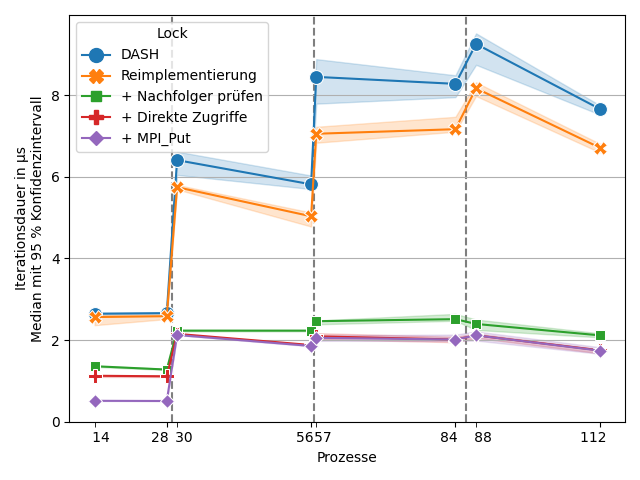
\includegraphics[width=\textwidth]{../../Dokumentation/Latex/Bilder/benchmarks/intelmpi/dash-optimization/ECSB-latency}
            \caption{ECSB}
        \end{figure}
    \end{minipage}
\end{frame}

\begin{frame}{Optimierung von \texttt{dash::Mutex}}
    \begin{minipage}{.49\textwidth}
        \begin{figure}
            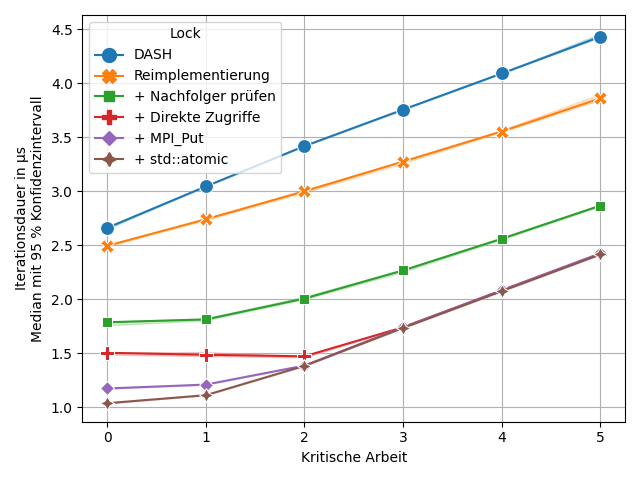
\includegraphics[width=\textwidth]{../../Dokumentation/Latex/Bilder/benchmarks/intelmpi/dash-optimization/CCWB-processes=28-latency}
            \caption{CCWB mit 28 Prozessen}
        \end{figure}
    \end{minipage}
    \begin{minipage}{.49\textwidth}
        \begin{figure}
            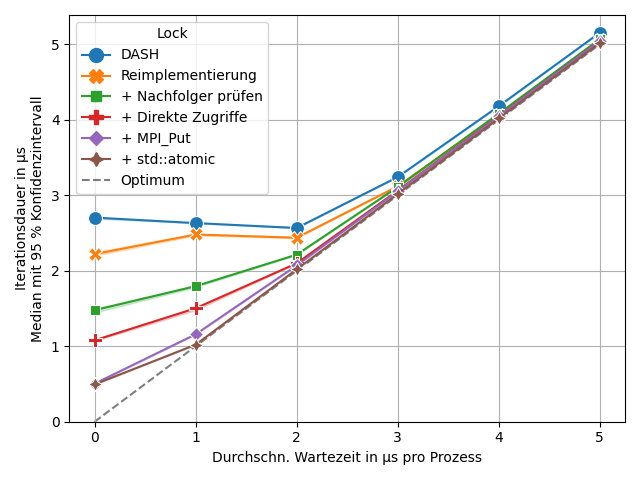
\includegraphics[width=\textwidth]{../../Dokumentation/Latex/Bilder/benchmarks/intelmpi/dash-optimization/WBAB-processes=28,mpi_progress=1-latency}
            \caption{WBAB mit 28 Prozessen}
        \end{figure}
    \end{minipage}
\end{frame}

\begin{frame}{Optimierung von \texttt{dash::Mutex}}
    \begin{minipage}{.49\textwidth}
        \begin{figure}
            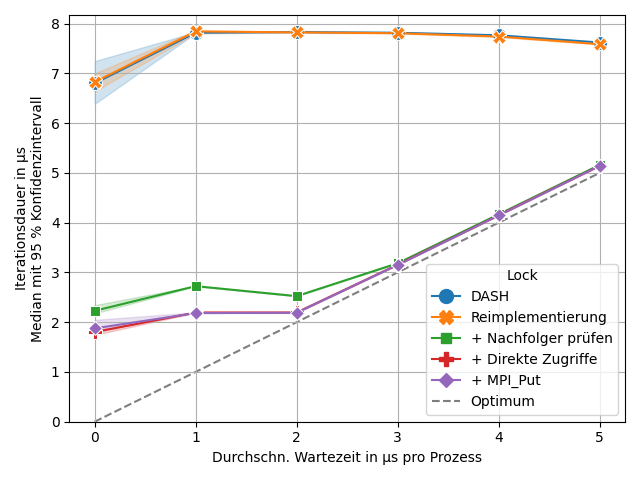
\includegraphics[width=\textwidth]{../../Dokumentation/Latex/Bilder/benchmarks/intelmpi/dash-optimization/WBAB-processes=112,mpi_progress=1-latency}
            \caption{WBAB mit 112 Prozessen}
        \end{figure}
    \end{minipage}
    \begin{minipage}{.49\textwidth}
        \begin{figure}
            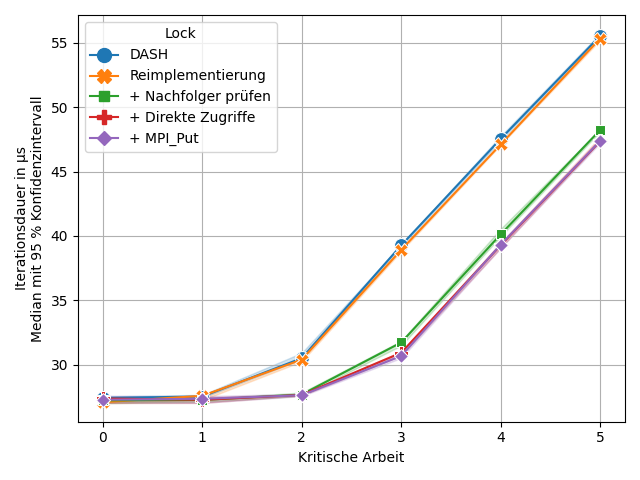
\includegraphics[width=\textwidth]{../../Dokumentation/Latex/Bilder/benchmarks/intelmpi/dash-optimization/CCWB-processes=112-latency}
            \caption{CCWB mit 112 Prozessen}
        \end{figure}
    \end{minipage}
\end{frame}

\begin{frame}{Cohort-Lock: Zähler-Optimierungen}
    \begin{minipage}{.49\textwidth}
        \begin{figure}
            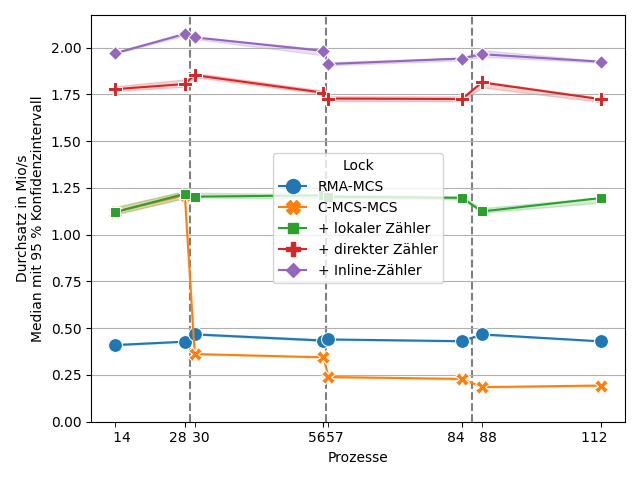
\includegraphics[width=\textwidth]{../../Dokumentation/Latex/Bilder/benchmarks/intelmpi/cohort-counter-optimization/ECSB-throughput}
            \caption{ECSB}
        \end{figure}
    \end{minipage}
    \begin{minipage}{.49\textwidth}
        \begin{figure}
            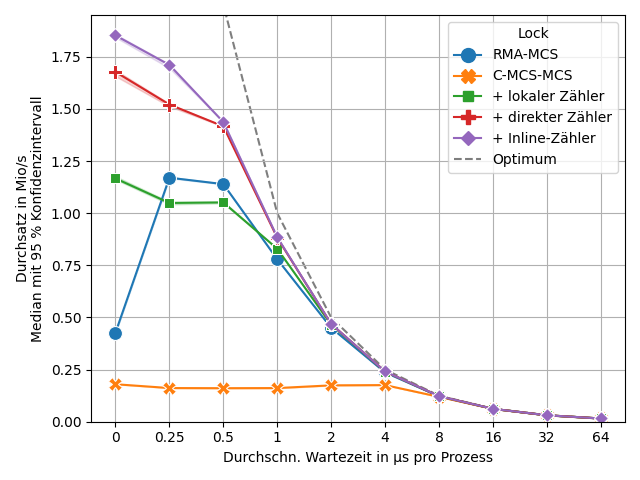
\includegraphics[width=\textwidth]{../../Dokumentation/Latex/Bilder/benchmarks/intelmpi/cohort-counter-optimization/WBAB-processes=112,mpi_progress=1-throughput}
            \caption{WBAB mit 112 Prozessen}
        \end{figure}
    \end{minipage}
\end{frame}

\begin{frame}{Cohort-Lock: Fairness verschiedener globaler und lokaler Locks}
    \begin{minipage}{.49\textwidth}
        \begin{figure}
            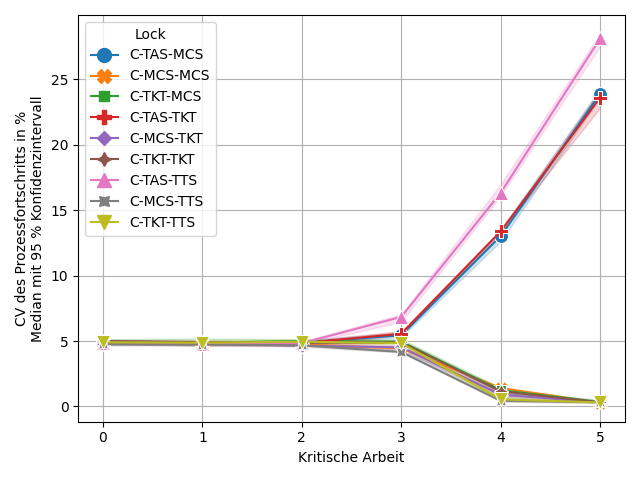
\includegraphics[width=\textwidth]{../../Dokumentation/Latex/Bilder/benchmarks/intelmpi/cohort-mcs-spin-tkt/CCWB-processes=112-fairness}
            \caption{CCWB Fairness}
        \end{figure}
    \end{minipage}
    \begin{minipage}{.49\textwidth}
        \begin{figure}
            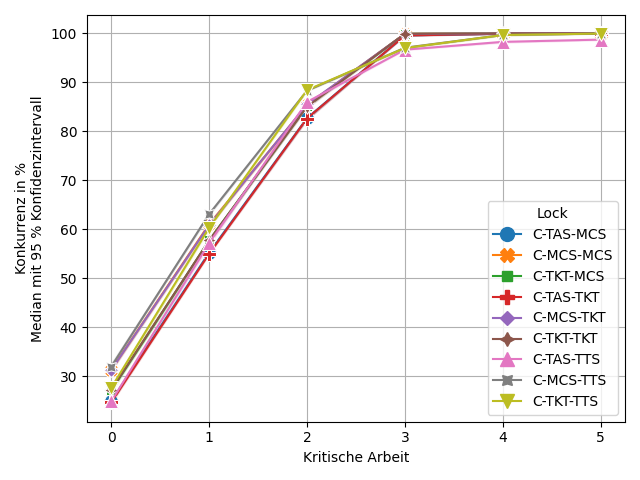
\includegraphics[width=\textwidth]{../../Dokumentation/Latex/Bilder/benchmarks/intelmpi/cohort-mcs-spin-tkt/CCWB-processes=112-contention}
            \caption{CCWB Konkurrenz}
        \end{figure}
    \end{minipage}
\end{frame}

\begin{frame}{RH-Lock}
    \begin{itemize}
        \item Basiert auf \textit{Test-and-Set} (TAS)-Locks für lokale Lockübergaben
        \item und \textit{Test-and-Test-and-Set} (TTS)-Locks für entfernte Lockübergaben
        \item Beides sind sehr unfaire Locks \pause
        \item[$\Rightarrow$] Auch der RH-Lock ist sehr unfair
    \end{itemize}
\end{frame}

\begin{frame}{RH-Lock Evaluation}
    \begin{minipage}{.49\textwidth}
        \begin{figure}
            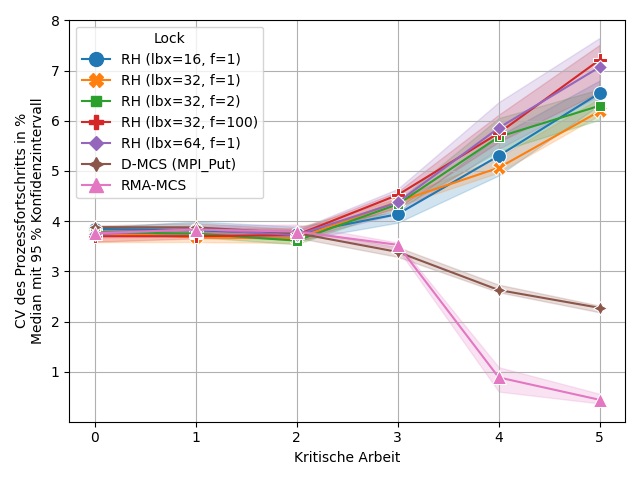
\includegraphics[width=\textwidth]{../../Dokumentation/Latex/Bilder/benchmarks/intelmpi/rh/CCWB-processes=112-fairness}
            \caption{CCWB Fairness}
        \end{figure}
    \end{minipage}
    \begin{minipage}{.49\textwidth}
        \begin{figure}
            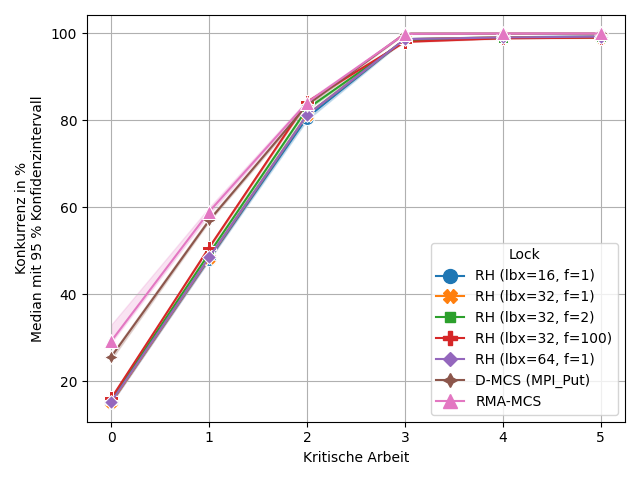
\includegraphics[width=\textwidth]{../../Dokumentation/Latex/Bilder/benchmarks/intelmpi/rh/CCWB-processes=112-contention}
            \caption{CCWB Konkurrenz}
        \end{figure}
    \end{minipage}
\end{frame}

\begin{frame}{SHFL-Lock}
    \begin{itemize}
        \item Nutzt einen TTS-Lock für den schnellen Pfad
        \item und einen MCS-Lock \cite{MCS-Lock} für den langsamen Pfad
        \item Prozesse in der MCS-Warteschlange werden nach NUMA-Knoten gruppiert
    \end{itemize}
\end{frame}

\begin{frame}{SHFL-Lock Evaluation}
    \begin{minipage}{.49\textwidth}
        \begin{figure}
            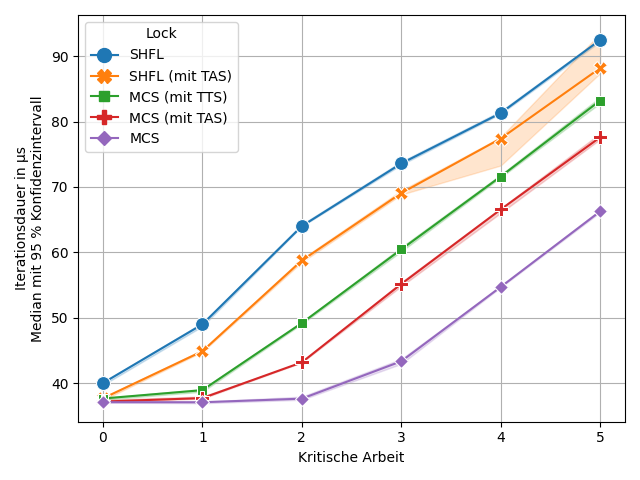
\includegraphics[width=\textwidth]{../../Dokumentation/Latex/Bilder/benchmarks/intelmpi/shfl/CCWB-processes=112-latency}
            \caption{CCWB mit 112 Prozessen}
        \end{figure}
    \end{minipage}
    \begin{minipage}{.49\textwidth}
        \begin{figure}
            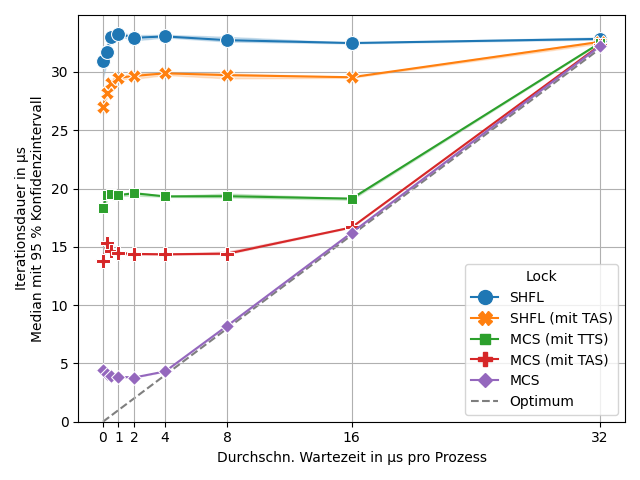
\includegraphics[width=\textwidth]{../../Dokumentation/Latex/Bilder/benchmarks/intelmpi/shfl/WBAB-processes=112,mpi_progress=1-latency}
            \caption{WBAB mit 112 Prozessen}
        \end{figure}
    \end{minipage}
\end{frame}

\end{document}
